%%%%%%%%%%%%%%%%%%%%%%%%%%%%%%%%
%------------------------------%
%%%%%%%%%%%%%%%%%%%%%%%%%%%%%%%%
\section*{Supplementary materials}
%%%%%%%%%%%%%%%%%%%%%%%%%%%%%%%%
%------------------------------%
%%%%%%%%%%%%%%%%%%%%%%%%%%%%%%%%

% 1D LINEAR ADMIXTURE KINSHIP
\begin{figure}[H]
    \centering
    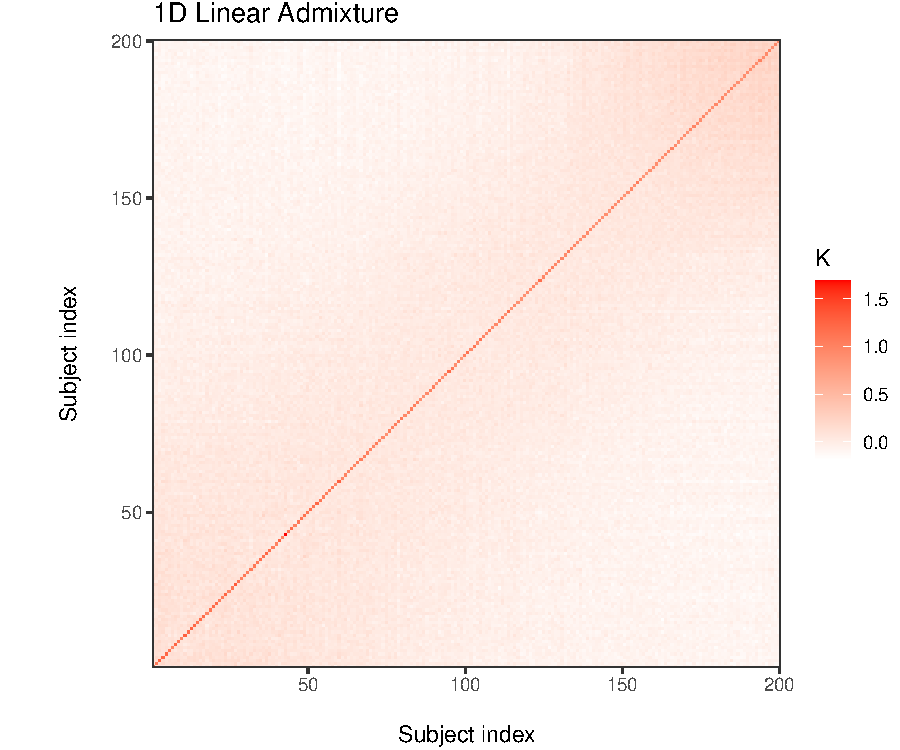
\includegraphics[scale = 1]{figures/figure_07.pdf}
    \caption{1D Linear Admixture with coarse subpopulation structure (4 subpopulations, 50 subjects per subpopulation), RRM.}
    \label{fig:admixed}
\end{figure}

% INDEPENDENT SUBPOPULATIONS, COARSE, KINSHIP
\begin{figure}[H]
    \centering
    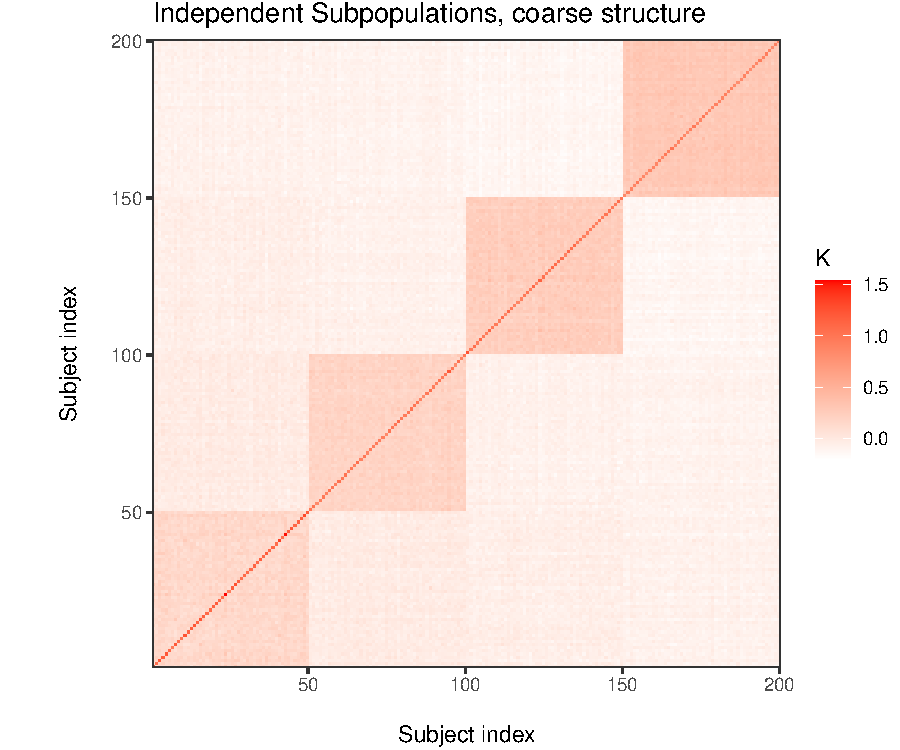
\includegraphics[scale = 1]{figures/figure_08.pdf}
    \caption{Independent Subpopulations with coarse subpopulation structure (4 subpopulations, 50 subjects per subpopulation), RRM.}
    \label{fig:indep_coarse}
\end{figure}

% INDEPENDENT SUBPOPULATIONS, FINE, KINSHIP
\begin{figure}[H]
    \centering
    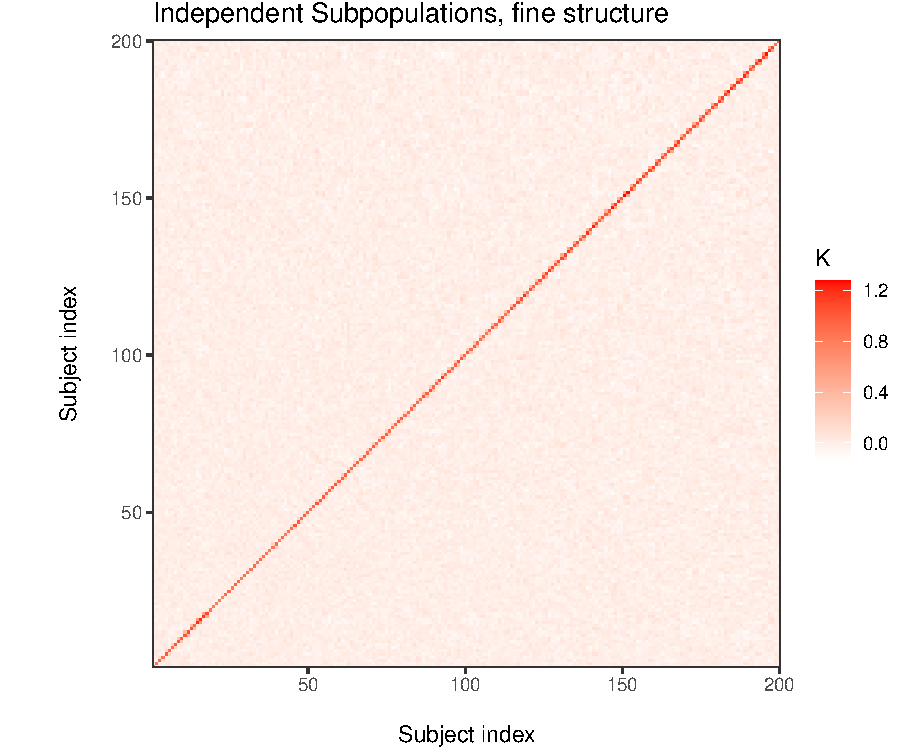
\includegraphics[scale = 1]{figures/figure_09.pdf}
    \caption{Independent Subpopulations with fine subpopulation structure (100 subpopulations, 2 subjects per subpopulation), RRM.}
    \label{fig:indep_fine}
\end{figure}

% EMPIRICAL KINSHIP
\begin{figure}[H]
    \centering
    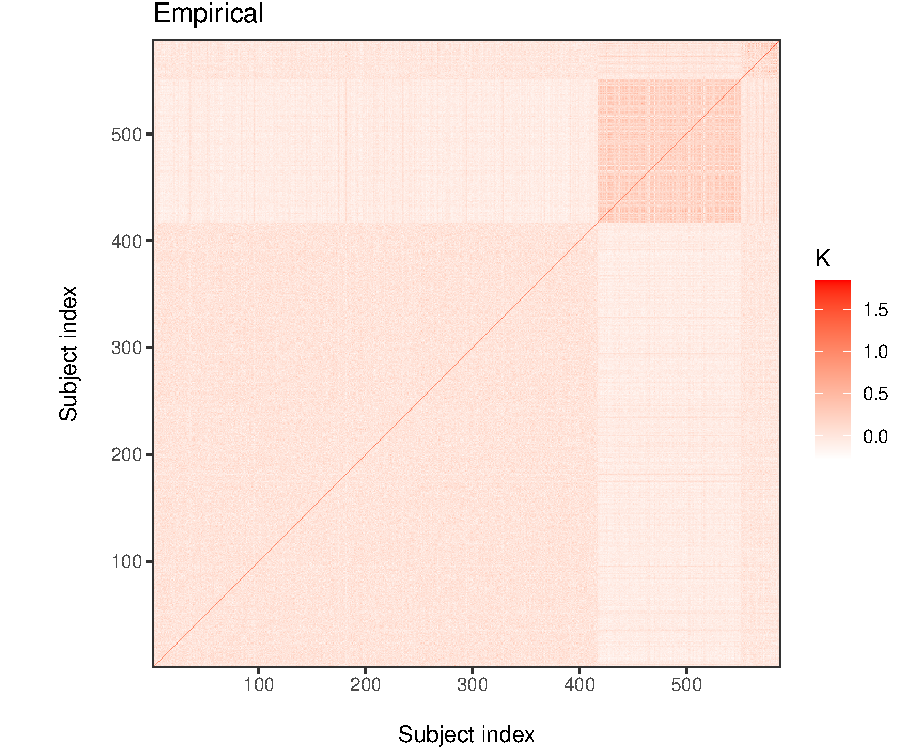
\includegraphics[scale = 1]{figures/figure_10.pdf}
    \caption{Empirical data with three subpopulations, Caucasian ($n = 417$), African American ($n = 134$), and Hispanic ($n = 37$), RRM.}
    \label{fig:empirical}
\end{figure}

\begin{figure}[H]
    \centering
    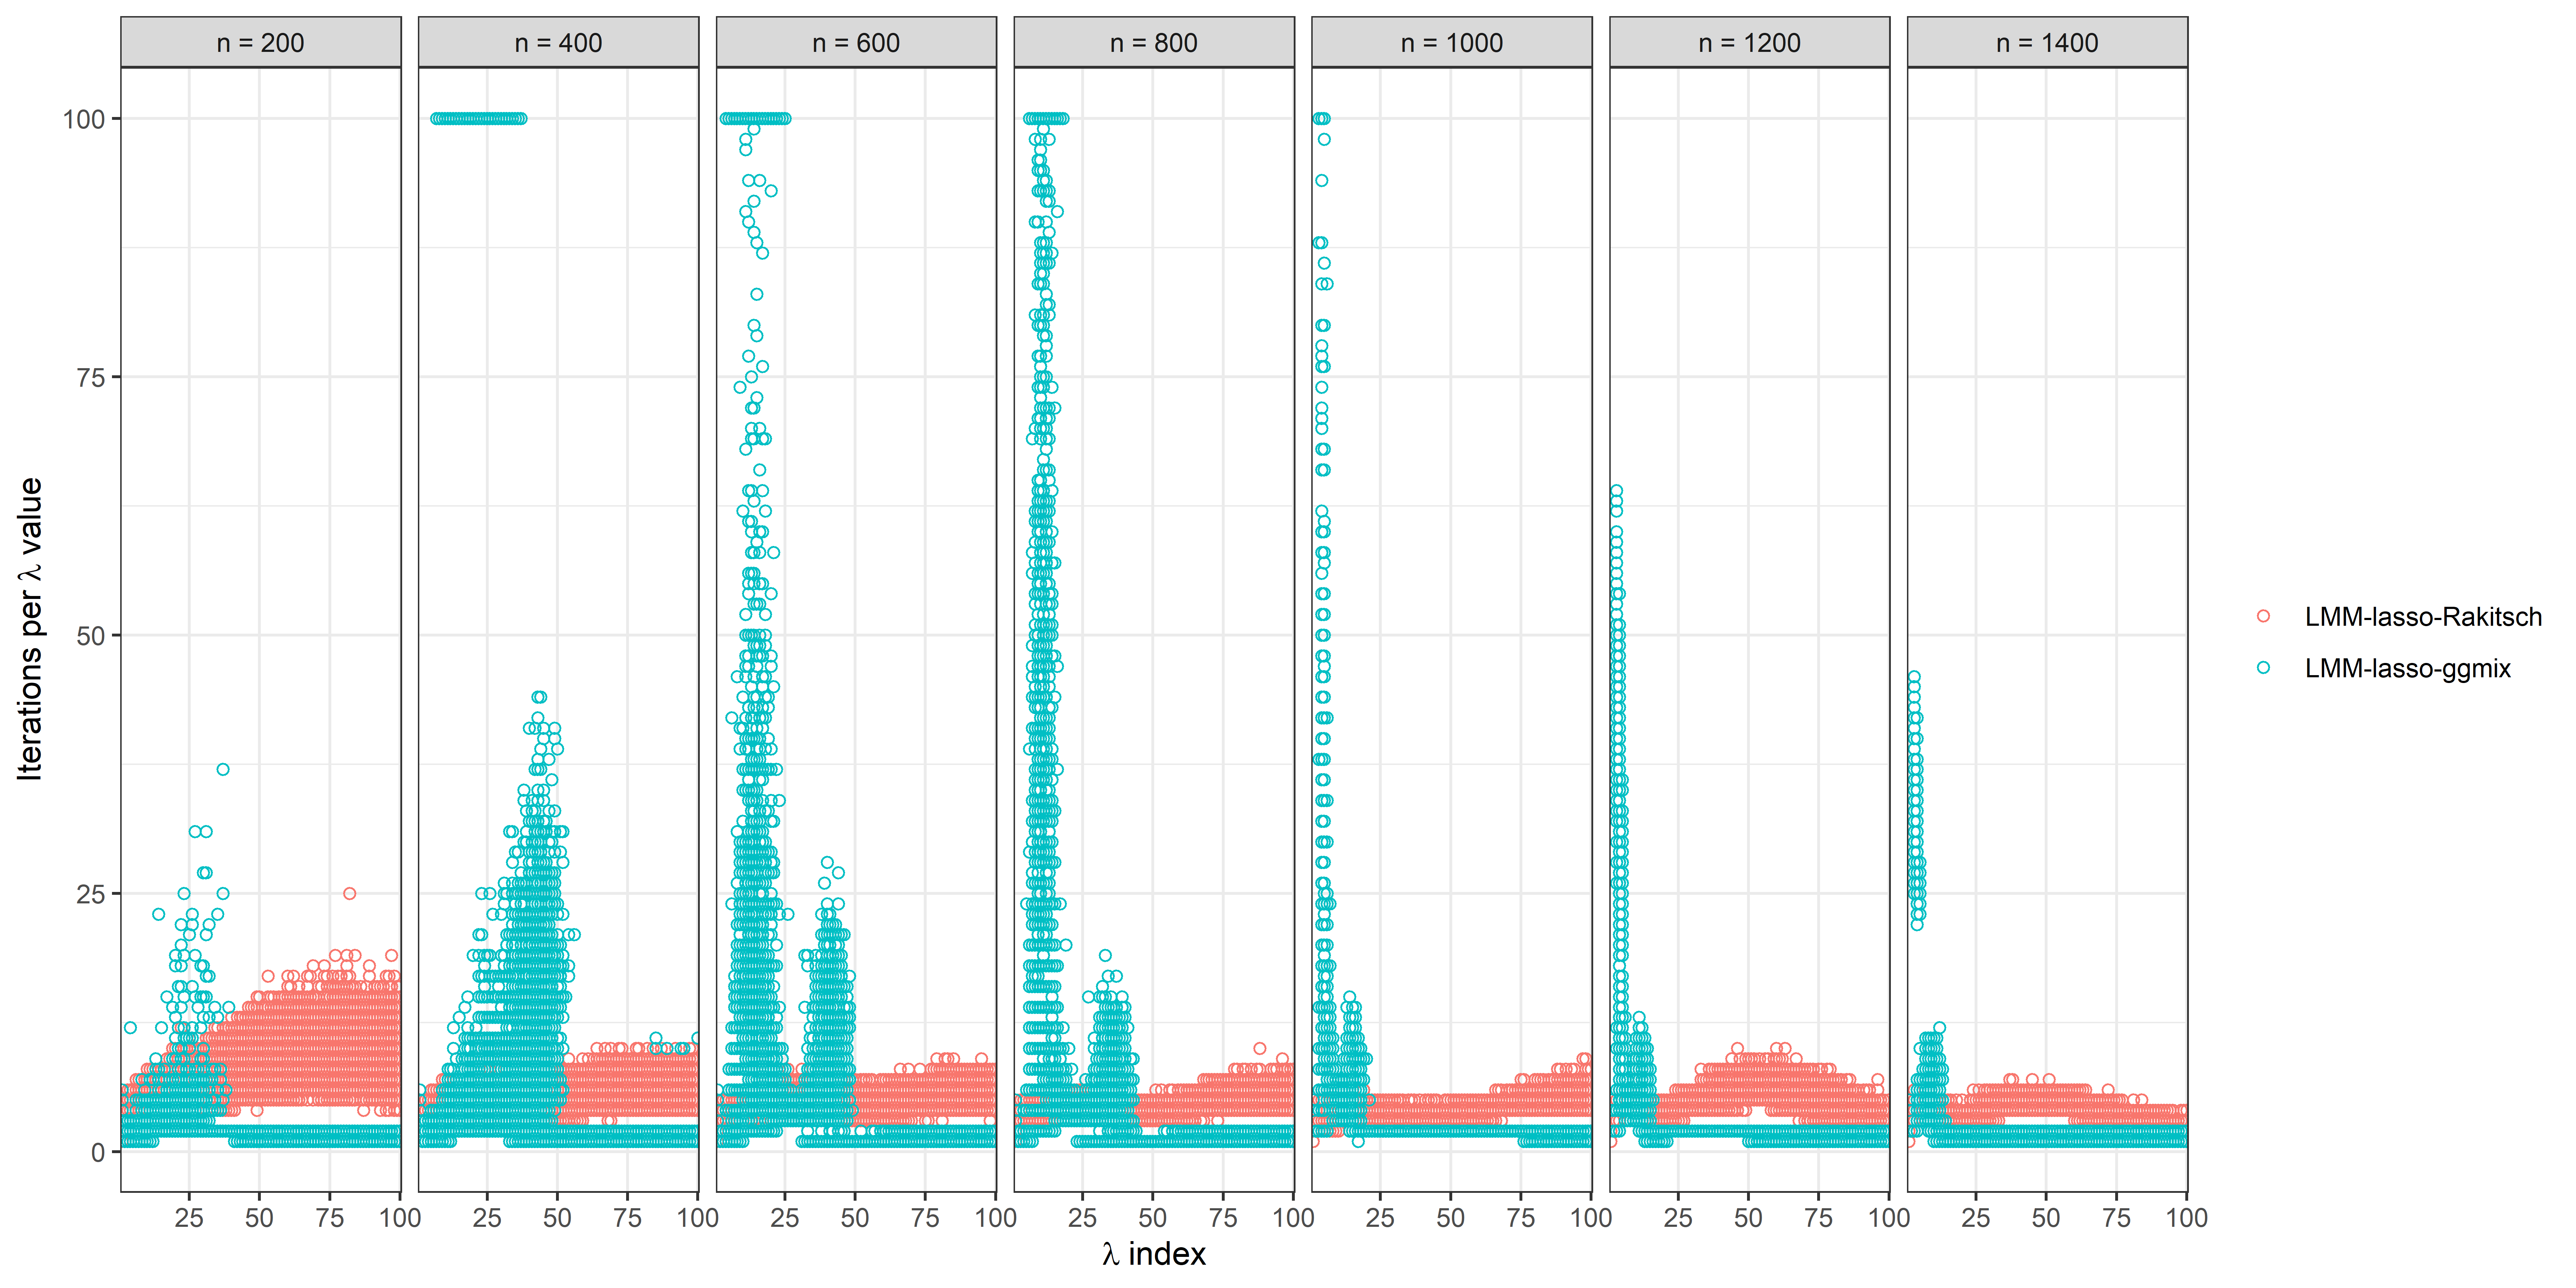
\includegraphics[width=\textwidth]{figures/figure_11.pdf}
    \caption{Number of iterations per $\lambda$ value for LMM-lasso-Rakitsch and LMM-lasso-ggmix across varying sample sizes with Independent Subpopulations data, coarse subpopulation structure, $\eta = 0.8$, and $\xi = 0.8$, and dichotomous-discordant environmental effect structure. Note that 100 is the maximum number of iterations for both implementations of LMM-lasso, so that numerous incidences of 100 iterations may indicate lack of model convergence.}
    \label{fig:niter}
\end{figure}
